\documentclass[letterpaper, 10pt]{article}

\usepackage{amsfonts}
\usepackage{amsmath}
\usepackage{hyperref}
\usepackage{xcolor}
\usepackage{graphicx}
\usepackage{tikz}
\usetikzlibrary{arrows}
\usetikzlibrary{decorations}
\usepackage{geometry}
\usepackage{listings}
\usepackage{algorithm}
\usepackage{algorithmicx}
\usepackage{algpseudocode}

\geometry{left=1.5cm,right=1.5cm,top=1.5cm,bottom=1.5cm}
\hypersetup{
	colorlinks, linkcolor=red, anchorcolor=blue, citecolor=purple
}

\newcommand{\qbar}{\rangle}
\newcommand{\qket}{\langle}

\begin{document}

\title{Restricted Boltzmann Machine}
\author{}
\date{\today}
\maketitle
\tableofcontents

\vskip 6cm
\begin{figure}[htbp]
\begin{center}
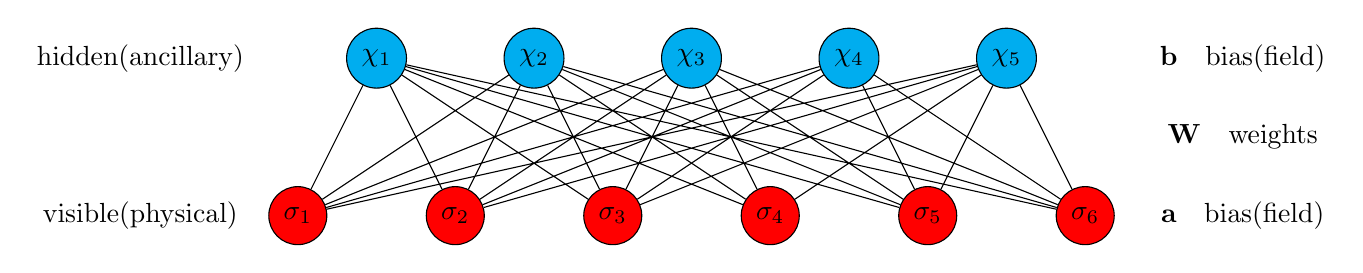
\begin{tikzpicture}
	\draw (7,-1) node {\textbf{a}\quad{}\textrm{bias(field)}} (7,0) node {\textbf{W}\quad{}\textrm{weights}} (7,1) node {\textbf{b}\quad{}\textrm{bias(field)}};
	\draw (-7,-1) node {\textrm{visible(physical)}} (-7,1) node {\textrm{hidden(ancillary)}};
	\tikzstyle{every node}=[draw,shape=circle,fill=red];
	\node (s1) at (-5,-1) {$\sigma_1$};
	\node (s2) at (-3,-1) {$\sigma_2$};
	\node (s3) at (-1,-1) {$\sigma_3$};
	\node (s4) at (1,-1) {$\sigma_4$};
	\node (s5) at (3,-1) {$\sigma_5$};
	\node (s6) at (5,-1) {$\sigma_6$};
	\tikzstyle{every node}=[draw,shape=circle,fill=cyan];
	\node (h1) at (-4,1) {$\chi_1$};
	\node (h2) at (-2,1) {$\chi_2$};
	\node (h3) at (0,1) {$\chi_3$};
	\node (h4) at (2,1) {$\chi_4$};
	\node (h5) at (4,1) {$\chi_5$};
	\draw 	(s1)--(h1) (s1)--(h2) (s1)--(h3) (s1)--(h4) (s1)--(h5)
			(s2)--(h1) (s2)--(h2) (s2)--(h3) (s2)--(h4) (s2)--(h5)
			(s3)--(h1) (s3)--(h2) (s3)--(h3) (s3)--(h4) (s3)--(h5)
			(s4)--(h1) (s4)--(h2) (s4)--(h3) (s5)--(h4) (s4)--(h5)
			(s5)--(h1) (s5)--(h2) (s5)--(h3) (s5)--(h4) (s5)--(h5)
			(s6)--(h1) (s6)--(h2) (s6)--(h3) (s6)--(h4) (s6)--(h5);
\end{tikzpicture}
\end{center}
\end{figure}

\newpage
\setcounter{page}{1}


\section{Introduction}

The main task of Machine Learning(ML) is learning from data and making predictions. There are three main steps in ML:
\begin{itemize}
	\item[1)]
	Collecting the training data set, usually from experiments, our daily life, etc;
	\item[2)]
	Finding a set of functions(also called model, which depends on a set of parameters) that is used to represent the law behind the data set;
	\item[3)]
	Defining a loss function to measure the goodness of your function, given certain parameter value, and find the best parameter value to minimize the loss function.
\end{itemize}
Considerations on each step can lead to methods with very different models and task-oriented algorithms.


\section[Basic Concepts \& Application]{Basic Concepts \& Application\cite{{melko2016prb},{fischer2012tb}}}

\subsection{Basic Concepts}
Restricted Boltzmann Machine(RBM) is a natural model for studing statistical physics, which can be used to learn the probability distribution of a data set. For a particular configuration $(\vec{\sigma}, \vec{\chi}) \in \{0,1\}^{N+M}$ , the RBM gives the joint distribution:
\begin{equation}
p(\vec{\sigma},\vec{\chi}) = \frac{1}{Z} \exp{(-E(\vec{\sigma},\vec{\chi}))},
\end{equation}
where the corresponding energy is defined as:
\begin{equation}
E(\vec{\sigma},\vec{\chi}) = - \sum_{i=1}^{M} b_i \chi_i - \sum_{j=1}^{N} a_j \sigma_j - \sum_{i,j} W_{ij} \chi_i \sigma_j,
\end{equation}
and $Z = \sum_{\vec{\sigma},\vec{\chi}} \exp{(-E(\vec{\sigma},\vec{\chi}))}$ is the so-called partition function which is essential to meet the normalization condition. Then we can get the marginal distribution for the physical configuration \{$\vec{\sigma}$\}:
\begin{equation}
p(\vec{\sigma}) = \sum_{\vec{\chi}} p(\vec{\sigma},\vec{\chi}) =  \frac{1}{Z} \exp{( {\color{red}{\sum_{j} a_j \sigma_j}} + {\color{cyan}{\sum_i \ln{( 1 + \exp{( b_i + \sum_j W_{ij} \sigma_j )} )}}} )} = \frac{1}{Z} \exp{( - \mathcal{E}(\vec{\sigma}) )},  \label{eq:eq1}
\end{equation}
and the {\color{red}{red}} part is just the mean field term, while the {\color{cyan}{cyan}} part, which is nonlinear, can capture the correlations. This makes RBM a powerful representation of a very complex probability distribution(indeed, any distribution with enough hidden units). Furthermore, we can calculate conditional distributions using Bayes's theorem as follows:
\begin{eqnarray*}
p(\vec{\sigma}|\vec{\chi}) & = &	\frac{\exp{(-E(\vec{\sigma},\vec{\chi}))}/Z}{\sum_{\vec{\sigma}} \exp{(-E(\vec{\sigma},\vec{\chi}))}/Z} \quad{} \textrm{insert the definition of energy $E(\vec{\sigma},\vec{\chi})$} \\
	& = & \frac{\prod_{j=1}^{N} \exp{(a_j \sigma_j + \sum_i W_{ij} \chi_i \sigma_j)}}{\prod_{j=1}^{N} (1 + \exp(a_j + \sum_i W_{ij} \chi_i))} \\
	& = & \prod_{j=1}^{N} \frac{\exp{(a_j \sigma_j + \sum_i W_{ij} \chi_i \sigma_j)}}{1+\exp{(a_j + \sum_i W_{ij} \chi_i)}}\,. \\
\end{eqnarray*}
We can hence reformulate the conditional distributions in a `decomposed' way(similar for $p(\vec{\chi}|\vec{\sigma})$)\footnote{Attention: the units in the same layer are independent variables when the other layer is fixed.}:
\begin{equation}
p(\vec{\sigma}|\vec{\chi}) = \prod_{j=1}^{N} p(\sigma_j | \vec{\chi}) \quad{} \mathrm{with} \quad{} p(\sigma_j=1 | \vec{\chi}) = \mathrm{sigmoid}(a_j + \sum_i W_{ij}\chi_i)\,; \label{eq:eq2}
\end{equation}
\begin{equation}
p(\vec{\chi}|\vec{\sigma}) = \prod_{i=1}^{M} p(\chi_i | \vec{\sigma}) \quad{} \mathrm{with} \quad{} p(\chi_i=1 | \vec{\sigma}) = \mathrm{sigmoid}(b_i + \sum_j W_{ij}\sigma_j)\,.\label{eq:eq3}
\end{equation}
The sigmoid function is defined as: $\mathrm{sigmoid}(x) = 1/(1+\exp{(-x)})$\footnote{In practical programming, $\exp(-x)$ may cause overflow. There is another safer version for the sigmoid function as: $(1+\tanh{(x/2)})/2$, which is preferred.}. An attractive fact about RBM is that: given any configuration $\vec{\sigma}$ as input, we can generate a data set(obey the distribution \ref{eq:eq1}) from Markov Chain Monte Carlo(MCMC) using the update rules \ref{eq:eq2} and \ref{eq:eq3}.

\subsection{Application}
Our aim is learning the thermodynamics of a classical spin system, and all we need to know is the partition function(Ising model for example):
\begin{equation}
Z(\beta) = \sum_{\vec{\sigma}} \exp{( -\beta E(\vec{\sigma}) )} \quad{} \mathrm{with} \quad{} E(\vec{\sigma}) = -J \sum_{<i,j>} \sigma_i \sigma_j.
\end{equation}
However, it is not practical to calculate it for a general model.  One can alternatively sample a data set from the corresponding distribution $q(\vec{\sigma}) = \exp{( -\beta E(\vec{\sigma}) )} / Z(\beta)$ and average the quantity interested over the data set. Here, we generate the data set(training set $\mathcal{D}$) via conventional Monte Carlo Simulation and train the RBM to learn the probability distribution $q(\vec{\sigma})$ hidden in the data set, finally we sample from the trained RBM and calculate the physical quantities. Thus, we need to find parameter value(namely \textbf{W}, \textbf{b}, \textbf{c}) which makes the RBM represent the distribution $q(\vec{\sigma})$ best. Kullback Leibler(KL) divergence is a measure of the distance between two distributions\footnote{$-\mathbb{KL}(q||p) = \sum_{\vec{\sigma}} q(\vec{\sigma}) \ln{ \frac{p(\vec{\sigma})}{q(\vec{\sigma})} } \leq \ln \sum_{\vec{\sigma}} q(\vec{\sigma}) \frac{p(\vec{\sigma})}{q(\vec{\sigma})} = 0$, which uses the Jensen's inequality, and the equality can be obtained via $p(\vec{\sigma})/q(\vec{\sigma}) = \text{const}$, together with the normalization condition, we finally arrive at: $\forall \vec{\sigma}, q(\vec{\sigma}) = p(\vec{\sigma})$.}:
\begin{eqnarray*}
\mathbb{KL}(q||p) & = & \sum_{\vec{\sigma}\,\,\textrm{for all}} q(\vec{\sigma}) \ln{ \frac{q(\vec{\sigma})}{p(\vec{\sigma})} } \quad{} \textrm{be zero iff } q(\vec{\sigma}) = p(\vec{\sigma}) \,\, \textrm{for all }\vec{\sigma} \\
	& = & \sum_{\vec{\sigma}\,\,\textrm{for all}} q(\vec{\sigma}) \ln{q(\vec{\sigma})} - \!\!\sum_{\vec{\sigma}\,\,\textrm{for all}} {\color{cyan}{q(\vec{\sigma})}} \ln{p(\vec{\sigma})} \quad{} \textrm{the first term is fixed by the true distribution} \\
	& \sim & - \!\!\sum_{\vec{\sigma}\,\,\textrm{for all}} {\color{cyan}{\frac{1}{| \mathcal{D} |} \sum_{\vec{\sigma}' \in \mathcal{D}} \delta_{\vec{\sigma},\vec{\sigma}'}}} \ln{p(\vec{\sigma})} \quad{} \textrm{note that} \,\, q(\vec{\sigma}) \,\, \textrm{can be estimated from the data set $\mathcal{D}$} \\
	& = & - \frac{1}{|\mathcal{D}|} \sum_{\vec{\sigma} \in \mathcal{D}} \ln p(\vec{\sigma}) \quad{} \textrm{note that the term } \sum_{\vec{\sigma} \in \mathcal{D}} \ln p(\vec{\sigma}) = \ln \prod_{\vec{\sigma} \in \mathcal{D}} p(\vec{\sigma}) \,\, \textrm{is also known as log-likelihood.}
\end{eqnarray*}
The most common strategy to minimize the KL divergence(our loss function) is using Stochastic Gradient Descent(SGD). Thus we need to calculate the derivatives of KL divergence with respect to RBM parameters $\vec{\lambda}$(attention: we write \{\textbf{W}, \textbf{b}, \textbf{c}\} as $\vec{\lambda}$):
\begin{equation}
\nabla_{\vec{\lambda}} \, \mathbb{KL}(q||p) = - \frac{1}{|\mathcal{D}|} \sum_{\vec{\sigma} \in \mathcal{D}} \nabla_{\vec{\lambda}} \, \ln{p_{\vec{\lambda}}(\vec{\sigma})}\,.\label{eq:eq10}
\end{equation}
Here we use $p_{\vec{\lambda}}(\vec{\sigma})$ to emphasize the parameter dependence of $p(\vec{\sigma})$. For each data $\vec{\sigma}^*$ in data set $\mathcal{D}$, we have:
\begin{eqnarray*}
\nabla_{\vec{\lambda}} \, \ln{p_{\vec{\lambda}}(\vec{\sigma}^*)} & = & \nabla_{\vec{\lambda}} \, \ln \frac{1}{Z_{\vec{\lambda}}} \sum_{\vec{\chi}} \exp{( - E_{\vec{\lambda}}(\vec{\sigma}^*,\vec{\chi}) )} \\
	& = & \nabla_{\vec{\lambda}} \, \ln \sum_{\vec{\chi}} \exp{( - E_{\vec{\lambda}}(\vec{\sigma}^*,\vec{\chi}) )} - \nabla_{\vec{\lambda}} \ln Z_{\vec{\lambda}} \\
	& = & - \frac{\sum_{\vec{\chi}} {\color{red}{\exp{( - E_{\vec{\lambda}}(\vec{\sigma}^*,\vec{\chi}) )}}} \nabla_{\vec{\lambda}} \, E_{\vec{\lambda}}(\vec{\sigma}^*,\vec{\chi})}{ {\color{red}{\sum_{\vec{\chi}} \exp{( - E_{\vec{\lambda}}(\vec{\sigma}^*,\vec{\chi}) )}}} } + \frac{\sum_{\vec{\sigma},\vec{\chi}} {\color{cyan}{\exp{(-E_{\vec{\lambda}}(\vec{\sigma},\vec{\chi}))}}} \nabla_{\vec{\lambda}} \, E_{\vec{\lambda}}(\vec{\sigma},\vec{\chi})}{ {\color{cyan}{\sum_{\vec{\sigma},\vec{\chi}} \exp{(-E_{\vec{\lambda}}(\vec{\sigma},\vec{\chi}))}}} } \\
	& = & - \sum_{\vec{\chi}} {\color{red}{p_{\vec{\lambda}}(\vec{\chi} | \vec{\sigma}^*)}} \nabla_{\vec{\lambda}} \, E_{\vec{\lambda}}(\vec{\sigma}^*,\vec{\chi}) + \sum_{\vec{\sigma},\vec{\chi}} {\color{cyan}{p_{\vec{\lambda}}(\vec{\sigma},\vec{\chi})}} \nabla_{\vec{\lambda}} \, E_{\vec{\lambda}}(\vec{\sigma},\vec{\chi}) \\
	& = & - \qket \nabla_{\vec{\lambda}} \, E_{\vec{\lambda}}(\vec{\sigma}^*,\vec{\chi})\qbar_{p_{\vec{\lambda}}(\vec{\chi} | \vec{\sigma}^*)} + \qket\nabla_{\vec{\lambda}} \, E_{\vec{\lambda}}(\vec{\sigma},\vec{\chi})\qbar_{p_{\vec{\lambda}}(\vec{\sigma},\vec{\chi})}\,,
\end{eqnarray*}
the first term is averaged over the conditional distribution for hidden layer given a certain $\vec{\sigma}^*$ which is easy to compute, while the second term is averaged over the distribution of the RBM which is difficult to calculate. Fortunately, the ML community have already proposed an efficient algorithm called contrastive divergence(CD) to estimate the second term. Here, we give more detail informations about the derivatives of KL divergence:
\begin{eqnarray}
\nabla_{W_{ij}} \, \ln{p_{\vec{\lambda}}(\vec{\sigma}^*)} & = & \qket \chi_i \sigma_j^* \qbar_{{p_{\vec{\lambda}}(\vec{\chi} | \vec{\sigma}^*)}} - \qket \chi_i \sigma_j \qbar_{{p_{\vec{\lambda}}(\vec{\chi},\vec{\sigma})}}\label{eq:eq4} \\
\nabla_{a_j} \, \ln{p_{\vec{\lambda}}(\vec{\sigma}^*)} & = & \qket \sigma_j^* \qbar_{{p_{\vec{\lambda}}(\vec{\chi} | \vec{\sigma}^*)}} - \qket \sigma_j \qbar_{{p_{\vec{\lambda}}(\vec{\chi},\vec{\sigma})}}\label{eq:eq5} \\
\nabla_{b_i} \, \ln{p_{\vec{\lambda}}(\vec{\sigma}^*)} & = & \qket \chi_i \qbar_{{p_{\vec{\lambda}}(\vec{\chi} | \vec{\sigma}^*)}} - \qket \chi_i \qbar_{{p_{\vec{\lambda}}(\vec{\chi},\vec{\sigma})}}\,.\label{eq:eq6}
\end{eqnarray}
Once we have calculated the derivatives of KL divergence given a certain parameter value, we can update the parameters with following rule:
\[ \vec{\lambda}^* = \vec{\lambda} - \eta \nabla_{\vec{\lambda}} \, \mathbb{KL}(\vec{\lambda})\,, \]
where the factor $\eta$ is the learning rate. The SGD will find the best parameter value automatically. Once we have trained a RBM, we can use MCMC method to sample from RBM which have learned the distribution of training data, and compute the physically relevant quantities as follows(denote sampled data set as: $\mathcal{S}$):
\[ \qket \mathcal{O} \qbar = \frac{1}{|\mathcal{S}|} \sum_{\vec{\sigma} \in \mathcal{S}} \mathcal{O}(\vec{\sigma})\,. \]


\section{Training Algorithm}

\subsection{Gibbs Sampling and Contrastive Divergence}
Now we have all the ingredients needed to train a RBM, and the main task is to calculate the values of \ref{eq:eq4}, \ref{eq:eq5} and \ref{eq:eq6}. Before we discuss the CD algorithm, it is essential to write these expressions more explicitly. For the first one:
\begin{eqnarray}
\nabla_{W_{ij}} \, \ln{p_{\vec{\lambda}}(\vec{\sigma}^*)} & = & {\color{cyan}{\sum_{\vec{\chi}} p_{\vec{\lambda}}(\vec{\chi} | \vec{\sigma}^*) \chi_i \sigma_j^*}} - \sum_{\vec{\sigma},\vec{\chi}} p_{\vec{\lambda}}(\vec{\sigma},\vec{\chi}) \chi_i \sigma_j \quad{} \textrm{using the identity}\,\, \ref{eq:eq3} \nonumber\\
	& = & ( \sum_{\chi_i} p_{\vec{\lambda}}(\chi_i | \vec{\sigma}^*) \chi_i \sigma_j^* ) \prod_{k \neq i} (\sum_{\chi_k} p_{\vec{\lambda}}(\chi_k | \vec{\sigma}^*)) - \sum_{\vec{\sigma},\vec{\chi}} p_{\vec{\lambda}}(\vec{\sigma},\vec{\chi}) \chi_i \sigma_j  \nonumber\\
	& = & \sum_{\chi_i} p_{\vec{\lambda}}(\chi_i | \vec{\sigma}^*) \chi_i \sigma_j^* - \sum_{\vec{\sigma}} p_{\vec{\lambda}}(\vec{\sigma}) {\color{cyan}{\sum_{\vec{\chi}} p_{\vec{\lambda}}(\vec{\chi} | \vec{\sigma}) \chi_i \sigma_j}} \nonumber\\
	& = & p_{\vec{\lambda}}(\chi_i=1 | \vec{\sigma}^*) \sigma_j^* - \sum_{\vec{\sigma}} p_{\vec{\lambda}}(\vec{\sigma}) p_{\vec{\lambda}}(\chi_i=1 | \vec{\sigma}) \sigma_j \nonumber\\
	& = & p_{\vec{\lambda}}(\chi_i=1 | \vec{\sigma}^*) \sigma_j^* - \qket p_{\vec{\lambda}}(\chi_i=1 | \vec{\sigma}) \sigma_j \qbar_{p_{\vec{\lambda}}(\vec{\sigma})}\label{eq:eq7}
\end{eqnarray}
Similarly, we have:
\begin{eqnarray}
\nabla_{a_j} \, \ln{p_{\vec{\lambda}}(\vec{\sigma}^*)} & = & \sigma_j^* - \qket \sigma_j \qbar_{p_{\vec{\lambda}}(\vec{\sigma})}\label{eq:eq8} \\
\nabla_{b_i} \, \ln{p_{\vec{\lambda}}(\vec{\sigma}^*)} & = & p_{\vec{\lambda}}(\chi_i=1 | \vec{\sigma}^*) - \qket p_{\vec{\lambda}}(\chi_i=1 | \vec{\sigma})\qbar_{p_{\vec{\lambda}}(\vec{\sigma})}\label{eq:eq9}
\end{eqnarray}
In order to get an average over distribution $p_{\vec{\lambda}}(\vec{\sigma})$, we can perform a Gibbs sampling\footnote{Start with a specific visible configuration $\vec{\sigma}^0$, we sample the hidden configuration $\vec{\chi}^0$ according to the probability \ref{eq:eq3} given $\vec{\sigma}^0$. Then we back to sample(reconstruct) the visible configuration $\vec{\sigma}^1$ according to the probability \ref{eq:eq2} given $\vec{\chi}^0$. If we do these sampling in order again and again, we will get a long sequence like(k-step Gibbs sampling): $\vec{\sigma}^0 \rightarrow \vec{\chi}^0 \rightarrow \vec{\sigma}^1 \rightarrow \vec{\chi}^1 \rightarrow \cdots \rightarrow \vec{\chi}^{k-1} \rightarrow \vec{\sigma}^k$. We refer to the ordered sampling procedure $\vec{\sigma} \rightarrow \vec{\chi} \rightarrow \vec{\sigma}$ as a single step of Gibbs sampling.}. However, this is very time-consuming,  for you have to do many steps(may be $\sim 10^3$ or larger) of Gibbs sampling before it reach the equilibrium(convergence). CD algorithm uses two tricks to circumvent this difficulty\footnote{The logic is that: our ultimate goal is getting a distribution $p_{\vec{\lambda}}(\vec{\sigma}) \sim q(\vec{\sigma}).$ If we start Gibbs sampling with a $\vec{\sigma}$ sampled from $q(\vec{\sigma})$, it should already arrive at the equilibrium in some sense.}: 1. start the Gibbs sampling with a $\vec{\sigma}$ from the training data set, not a random one; 2. do sampling after only a few steps of Gibbs sampling(in many cases, a single step is good enough!). In the spirit of CD algorithm, we can thus replace the average over $p_{\vec{\lambda}}(\vec{\sigma})$ in \ref{eq:eq7}, \ref{eq:eq8} and \ref{eq:eq9} with $p_{\vec{\lambda}}(\chi_i=1 | \vec{\sigma}^k) \sigma_j^k$,  $\sigma_j^k$ and $p_{\vec{\lambda}}(\chi_i=1 | \vec{\sigma}^k)$, where $\vec{\sigma}^k$ is sampled from $k$-step Gibbs sampling whose starting point is $\vec{\sigma}^*$\footnote{You may be confused and ask the question that: how you can replace the average over a distribution $p_{\vec{\lambda}}(\vec{\sigma})$ just by one $\vec{\sigma}$ sampled from it? The answer lies in the fact that our derivative of KL divergence includes an average(or sum) over the whole data set or a batch in SGD(see expression \ref{eq:eq10}). You may convince yourself that: this averaging process over training data set or batch indeed mimics the averaging process over the distribution $p_{\vec{\lambda}}(\vec{\sigma})$.}.

\subsection{Pseudocode For Training Algorithm}
Here I just give a detailed description of the whole training algorithm, see Algorithm \ref{al:rbm}.

\begin{algorithm}[htb]
	\caption{Training of RBM via SGD}\label{al:rbm}
	\begin{algorithmic}[1]
		\Require Data Set $\mathcal{D}$, RBM's Parameters $\{\textbf{W}, \textbf{a}, \textbf{b}\}$, Learning Rate $\eta$, Batch Size $bs$, Epoch $ep$, CD Order $k$, Visible Unit Number: $N$ and Hidden Unit Number: $M$.
		\Ensure $\{\textbf{W}^*, \textbf{a}^*, \textbf{b}^*\} = \mathop{\arg\min}_{\vec{\lambda}} \mathbb{KL}(q(\vec{\sigma})||p_{\vec{\lambda}}(\vec{\sigma}))$
		\State Initialize $\{\textbf{W}, \textbf{a}, \textbf{b}\}$. Each element in $\textbf{W}$ is sampled from a gaussian distribution: $W_{ij} \sim \mathcal{N}(0,1)/\sqrt(N+M)$, all the elements in $\textbf{a}, \textbf{b}$ are set to zero: $b_i \leftarrow 0, a_j \leftarrow 0$.
		\State Split $\mathcal{D}$ into batches $\mathcal{B}$ randomly, each is of size $bs$
		\For {$epoch$ in $range(1, ep)$}
			\For {each batch $B$ in $\mathcal{B}$}
				\State $\Delta W_{ij}, \Delta a_j, \Delta b_i$ are set to 0, for all $i, j$
				\For {each data $\vec{\sigma}$ in batch $B$}
					\State sample $\vec{\sigma}^k$ via $k$-step Gibbs sampling with $\vec{\sigma}$ as the starting configuration
					\State calculate $p(\chi_i=1|\vec{\sigma})$ and $p(\chi_i=1|\vec{\sigma}^k)$ for all $i$ via \ref{eq:eq2} and \ref{eq:eq3}
					\State $\Delta W_{ij} +\!\!= p(\chi_i=1|\vec{\sigma})*\sigma_j - p(\chi_i=1|\vec{\sigma}^k)*\sigma^k_j$
					\State $\Delta a_j +\!\!= \sigma_j - \sigma_j^k$
					\State $\Delta b_i +\!\!= p(\chi_i=1|\vec{\sigma}) - p(\chi_i=1|\vec{\sigma}^k)$
				\EndFor
				\State $W_{ij} \leftarrow W_{ij} + \eta * \Delta W_{ij} / bs$
				\State $a_j \leftarrow a_j + \eta * \Delta a_j / bs$
				\State $b_i \leftarrow b_i + \eta * \Delta b_i / bs$
			\EndFor
		\EndFor
	\end{algorithmic}
\end{algorithm}

\centering
\begin{thebibliography}{99}
\bibitem{melko2016prb} Learning Thermodynamics with Boltzmann Machines, G. Torlai, R.G. Melko, \href{https://arxiv.org/abs/1606.02718}{arXiv:1606.02718v1}
\bibitem{fischer2012tb} An Introduction to Restricted Boltzmann Machines, A. Fischer, C. Igel, \url{https://doi.org/10.1007/978-3-642-33275-3_2}

\end{thebibliography}

\end{document}
